\vspace{1.5cm}

En la figura~\figref{fig:fig_p21}, se muestra el circuito de la fuente de alimentación basado en el \textit{LM723} que armamos usando el mismo driver de corriente que la fuente original y ajustando los resistores de tal forma de que las características de tensión, limitación de corriente, etc, se parezcan lo mas posible al circuito original, los valores de compensación se toman de circuitos recomendados.\\
Con ese circuito, adecuadamente modificado, se repitieron las simulaciones para realizar la comparación pedida.\\

\vfill


\clearpage

\begin{figure}[H] %htb
\begin{center}
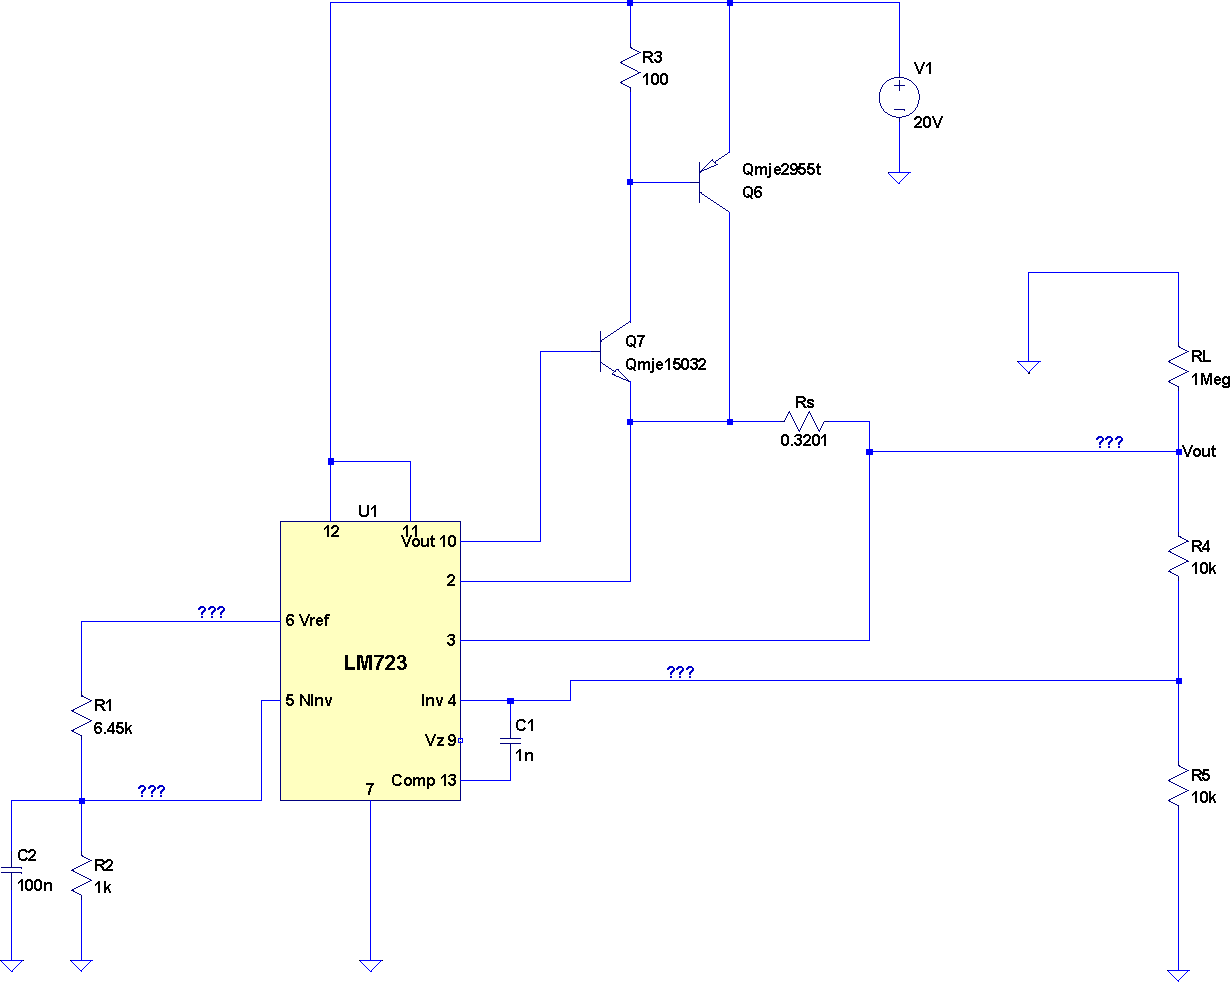
\includegraphics[width=1.2 \textwidth, angle=90]{./img/preguntas/p21.png}
\caption{\label{fig:fig_p21}\footnotesize{Rizado de entrada y salida.}}
\end{center}
\end{figure}

\clearpage